\chapter{Phase 1 - Dataset Engineering \& Lifecycle Strategy}
\setcounter{section}{0}
\renewcommand{\thesection}{\arabic{section}}
\label{chap:phase1-data}

\section{Chapter Introduction}
This chapter covers the critical ``Data Understanding'' and ``Data Preparation'' phases of the project, structured according to the CRISP-DM methodology \cite{ref:crisp-dm}. A core premise of this research is that model performance on industrial Neural Processing Units (NPUs) is fundamentally limited by data quality, not merely by the underlying network architecture. To achieve reliable deployment, the dataset must be meticulously engineered to meet strict hardware and accuracy constraints.

\subsection{CRISP-DM Methodology Mapping}
This phase is strictly aligned with the Cross-Industry Standard Process for Data Mining (CRISP-DM) framework. The ``Data Understanding'' phase involved an initial exploratory analysis of the warehouse environment, identifying the types of cameras available, their respective blind spots, and the typical frequency of safety incidents. We documented the baseline operational metrics, noting that on an average day, a warehouse might see hundreds of forklift-pedestrian interactions but zero actual fires. This extreme rarity of critical events heavily influenced our data collection strategy.

The subsequent ``Data Preparation'' phase, which forms the bulk of this chapter, focuses on transforming this raw understanding into a structured tensor format suitable for deep learning. This involved not only labeling the data but also designing a robust data pipeline that could handle the continuous influx of new footage. The CRISP-DM methodology emphasizes that data preparation is rarely a single step; it is an iterative process. As we transitioned into the modeling phase (Chapter 3), we frequently returned to this preparation phase to refine our labels based on the model's false-positive analyses.

\section{Raw Data Collection}
The data lifecycle began with raw data acquisition directly from the target industrial environment, utilizing a network of specialized industrial sensors and CCTV feeds. The initial state of the collected footage was unstructured and characterized by high informational entropy. It contained a wide variety of ``real-world'' labels capturing the chaotic dynamics of warehouse operations, personnel movement, and environmental noise, all recorded prior to any structured optimization.

To ensure the dataset accurately reflected the deployment environment, data was sampled across multiple shifts, varying lighting conditions (e.g., bright daylight through skylights, artificial night-time LED illumination), and diverse operational scenarios. High-definition 4K cameras were strategically positioned at operational choke points such as loading docks, main storage aisles, and blind intersections where forklift-to-pedestrian interactions are most frequent and dangerous. 

A critical challenge during this phase was managing the sheer volume of redundant temporal data. Continuous video feeds generated terabytes of footage where nothing of interest occurred. To mitigate this, a preliminary frame-extraction script was deployed to sample frames dynamically. During high-activity periods (e.g., active loading), frames were extracted at 2 frames per second (FPS), whereas during idle periods, the extraction rate dropped to 1 frame every 10 seconds. This intelligent sampling strategy drastically reduced storage overhead, eliminated sequential frame bias, and maximized the informational density of the raw dataset.

\section{The Pipeline Loop}
As illustrated in Figure~\ref{fig:pipeline-loop}, the project adopts a Data-Centric AI approach, where the focus remains on the iterative refinement of the dataset rather than static model training. Rather than following a strict linear progression, the data workflow was designed to harness the synergy between automated systems and human expertise.

\textbf{Continuous Ingestion:} Unlike traditional machine learning pipelines that rely on a static, one-time data upload, raw data is continuously fed into the system from the left side of the workflow. This ensures the model constantly adapts to the evolving reality of the warehouse floor.

\textbf{The ``Human-in-the-Loop'' (HITL) Element:} The pipeline integrates a semi-automated labeling loop, significantly reducing the temporal overhead of manual annotation while maintaining the high precision required for industrial safety applications. Utilizing Label Studio as the core annotation engine, this step creates a ``Gold Standard'' dataset where an AI model proposes initial labels, and the human engineer verifies and refines them.

\textbf{The Feedback Mechanism:} The circular arrows in the diagram represent a powerful acceleration mechanism. As the model's automated detection capabilities improve, it is increasingly trusted to auto-label incoming raw data. This symbiotic relationship creates a progressively faster development cycle.

\textbf{Deployment Integration:} The detection phase is not the final step. Instead, it feeds directly back into the data health check. By systematically identifying where the model is failing in deployment, the pipeline dictates exactly what kind of new data must be collected next. This circular architecture ensures that edge cases identified during the detection phase are re-ingested into the labeling queue, progressively hardening the model against false positives.

\begin{figure}[htbp]
\centering
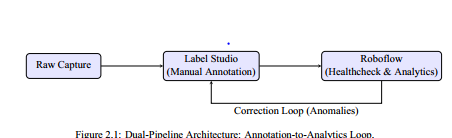
\includegraphics[width=0.9\textwidth]{dataannotationimages/diagramworkflow.PNG}
\caption{The Iterative Data Engineering Pipeline. This workflow illustrates the feedback loop between automated detection and manual verification (Label Studio), ensuring continuous dataset refinement before NPU deployment.}
\label{fig:pipeline-loop}
\end{figure}

\section{The Environment}
To manage the complexity of the raw data, a robust two-tool ecosystem was established. This environment bridged the gap between manual human annotation and automated dataset analytics. The selection of these specific tools was driven by the need for scalable, collaborative annotation and deep programmatic access to dataset metrics.

\begin{figure}[htbp]
\centering
\begin{minipage}{0.45\textwidth}
  \centering
  
\includegraphics[width=0.6\textwidth]{dataannotationimages/labelstudiologo.png}
  \caption{Label Studio (Annotation Workspace)}
\end{minipage}\hfill
\begin{minipage}{0.45\textwidth}
  \centering
  
\includegraphics[width=0.6\textwidth]{dataannotationimages/roboflowlogo.png}
  \caption{Roboflow (Management \& Analytics)}
\end{minipage}
\end{figure}

Label Studio was chosen for its highly customizable interface and support for complex annotation schemas, allowing the team to define strict guidelines for bounding box coordinates and object occlusion. Roboflow served as the central hub for dataset versioning, preprocessing, and exploratory data analysis (EDA). The API/Webhook integration between the two platforms enabled a seamless, automated MLOps workflow: once a batch of images was annotated in Label Studio, it was automatically pushed via API to Roboflow for immediate health checking. If Roboflow's analytics revealed severe class imbalances, the feedback was routed back to the collection phase to gather more targeted data, successfully closing the loop.

\section{Technical Implementation (Label Studio)}
\textbf{Label Studio} \cite{ref:labelstudio} was utilized to execute the annotation protocol. To ensure high-quality ground truth, annotators were required to create high-precision, tight bounding boxes around objects of interest.

\subsection{Configuration of the Annotation Environment}
The technical setup of the annotation environment was a critical first step before any manual labeling commenced. Rather than relying on ad-hoc configurations, the interface was strictly defined using a declarative XML/HTML labeling config. This configuration hardcoded the specific class vocabulary (e.g., `forklift`, `pedestrian`, `fire`) directly into the UI. This rigid setup ensures that every annotator follows the exact same class definitions, drastically reducing human error such as typos or the creation of unauthorized sub-classes.

Below is a snippet of the XML configuration used to define the labeling interface, illustrating how classes and their corresponding bounding box tools were programmatically enforced:

\begin{verbatim}
<View>
  <Image name="image" value="$image"/>
  <RectangleLabels name="label" toName="image">
    <Label value="forklift" background="#FF0000"/>
    <Label value="pedestrian" background="#00FF00"/>
    <Label value="fire" background="#FFA500"/>
  </RectangleLabels>
</View>
\end{verbatim}

Furthermore, the User Interface (UI) efficiency was paramount. The interface shown in Figure~\ref{fig:labelstudio-interface} is optimized for rapid, hotkey-based labeling. Annotators could toggle between classes, adjust bounding box coordinates, and navigate between frames without removing their hands from the keyboard. This level of ergonomic efficiency was absolutely necessary to handle the thousands of frames required to build an NPU-grade dataset within the project's timeline.

Finally, the interface features a visible "Audit" Trail. The list of images arrayed along the side and top of the workspace represents the "Task Queue." This queue provides a systematic way to track progress, ensuring that no raw data was inadvertently missed during the ingestion phase and that every frame was accounted for before the dataset was pushed to the next pipeline stage.

\begin{figure}[htbp]
\centering
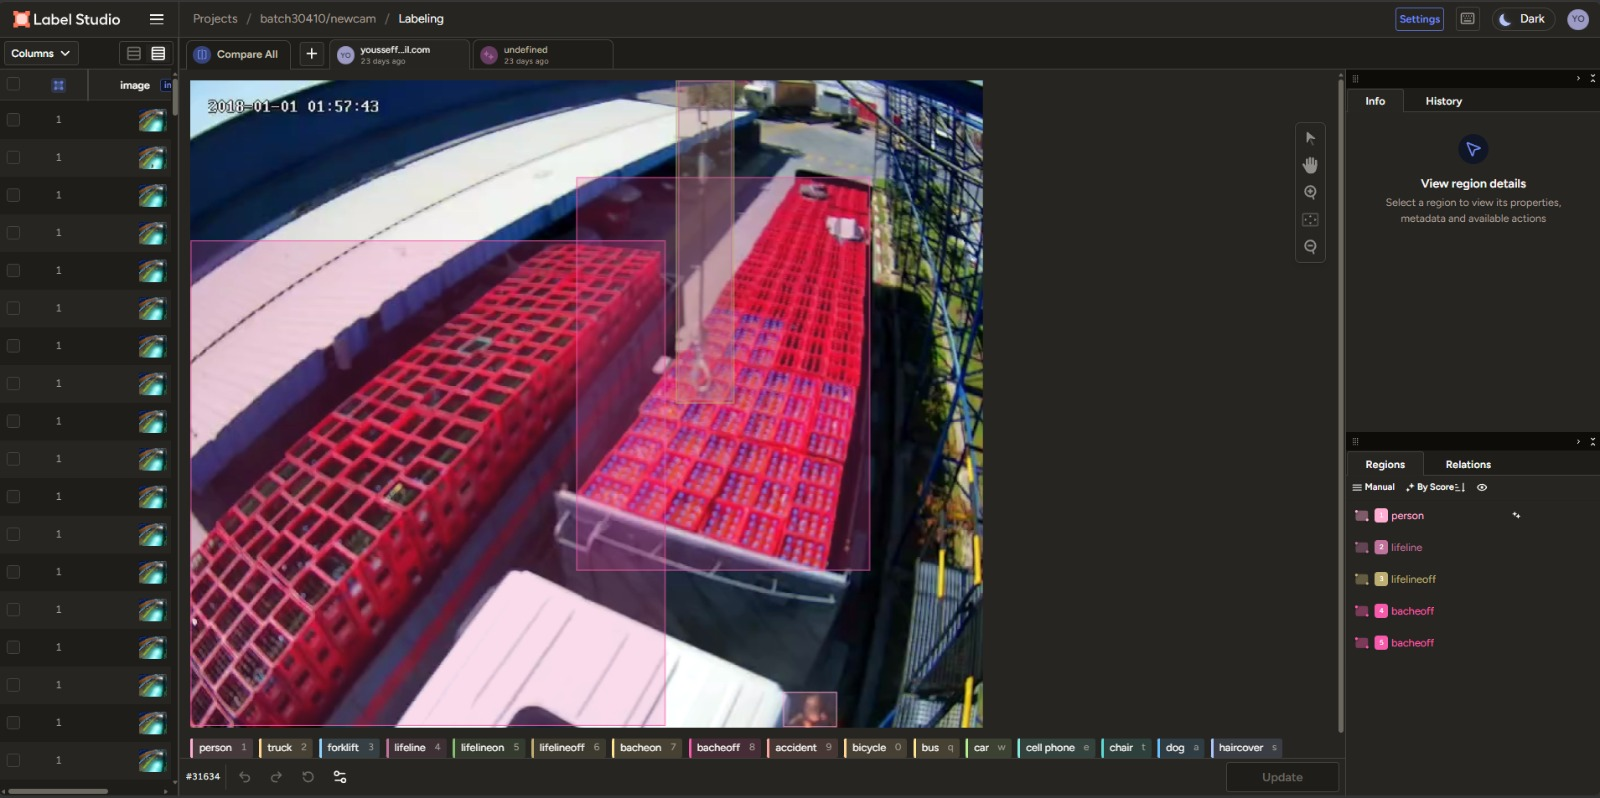
\includegraphics[width=1.0\textwidth]{dataannotationimages/labelstudiointerface.jpeg}
\caption{The Label Studio configuration interface, showcasing the task queue (Audit Trail) and the customized layout designed for rapid, hotkey-based annotation.}
\label{fig:labelstudio-interface}
\end{figure}

\subsection{Annotation Precision and Occlusion Handling}
The core of the annotation strategy was governed by a strict Bounding Box Protocol centered on "Tightness." For NPU optimization, it is not enough to simply draw a box around an object; the bounding boxes must be pixel-perfect. If a box is drawn too loosely, the model will inadvertently learn the background noise (e.g., concrete floors, racking shadows) as part of the object's visual signature. Moreover, loose bounding boxes severely distort the K-Means clustering algorithm used by YOLO to generate anchor box priors. Accurate anchor boxes are critical for the neural network's initial object localization phase, directly impacting the convergence speed and final inference performance on the NPU. By enforcing absolute tightness, we ensure the neural network's feature maps are densely packed with relevant semantic information.

Handling complex scenes was a daily challenge, as industrial warehouse environments are visually chaotic. Figure~\ref{fig:labelstudio-example2} illustrates a real-world scenario requiring careful handling of Occlusion (objects partially hidden by racks or other vehicles) and Truncation (objects partially out of frame). The protocol dictated that if more than 30\% of an object's core structure (e.g., the mast, the chassis, or the operator cabin of a forklift) was visible, it must be annotated, but flagged with a specific `occluded` metadata tag set to `true`. This allows the training pipeline to selectively weight these difficult examples during the later stages of training.

Another critical scenario involved the `fire` class. Early testing revealed that annotators were inconsistently labeling reflections of warning lights or bright sparks from welding as `fire`. To resolve this, the protocol was updated to require the presence of both a luminous core and a distinct smoke plume before an object could be labeled as `fire`. Furthermore, as illustrated in Figure~\ref{fig:label-studio-implementation}, the annotation interface allows for precise adjustments even for objects positioned in the far background, which might easily be missed by base models due to their distance and scale.

Following the manual labeling process, a rigorous Quality Control (QC) verification step was performed. This step involved cross-referencing labels across different lighting conditions-such as deep shadows in the warehouse aisles versus glare near loading docks-to ensure absolute label consistency regardless of photometric variations.

\begin{figure}[htbp]
\centering
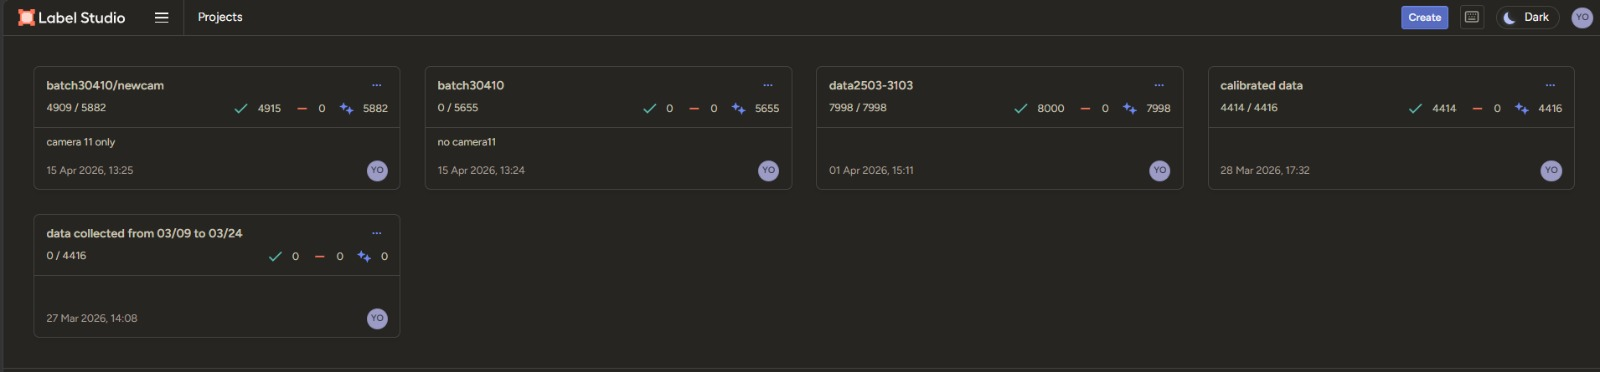
\includegraphics[width=1.0\textwidth]{dataannotationimages/labelstudioexample2.jpeg}
\caption{Label Studio interface demonstrating precision bounding boxes in a complex, occluded industrial scene.}
\label{fig:labelstudio-example2}
\end{figure}

\begin{figure}[htbp]
\centering
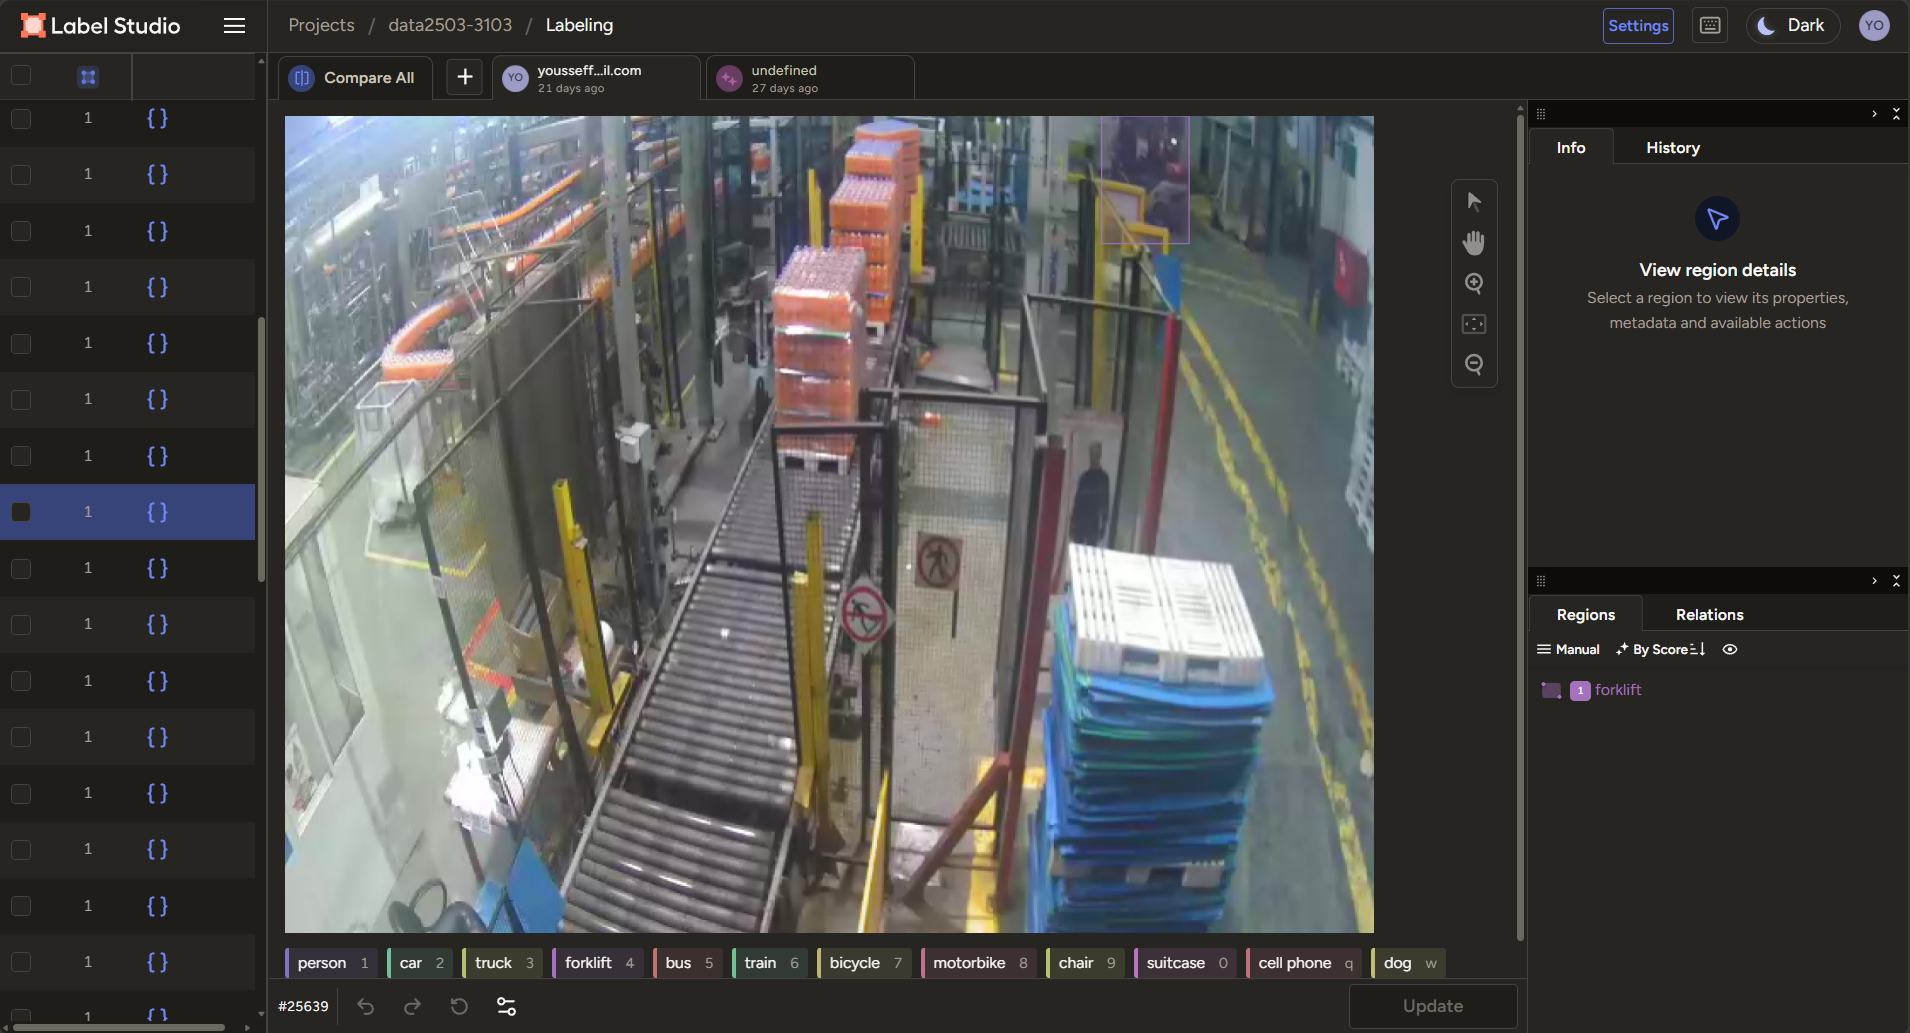
\includegraphics[width=1.0\textwidth]{dataannotationimages/labelstudio.png}
\caption{Label Studio interface demonstrating the high-precision bounding box implementation for distant, partially occluded objects (e.g., the forklift on the far top right).}
\label{fig:label-studio-implementation}
\end{figure}

\section{Data Filtering Strategy}
A critical ``Filtering Step'' was implemented to audit the raw labels before finalizing the dataset. The technical justification for this filtering is anchored in the hardware limitations of the deployment environment. NPUs possess strict SRAM and thermal constraints \cite{ref:efficientnet, ref:yolov8}. Training a model on an excessively broad vocabulary of highly imbalanced, granular classes would exceed these constraints and dilute the model's predictive focus. 

By systematically analyzing the variety of labels, strategic decisions were made regarding which classes to keep, merge, or discard, ensuring the dataset was optimized strictly for the project's primary safety and logistical objectives. For instance, the raw data contained separate labels for ``electric pallet jack'', ``reach truck'', and ``counterbalance forklift''. While these distinctions are visually identifiable, they all represent the same logistical hazard from a safety perspective. Therefore, these subclasses were merged into a single, robust \texttt{forklift} macro-class, providing the model with more diverse examples of a single concept.

Conversely, classes that appeared in less than 0.5\% of the frames and held no critical safety value (e.g., ``abandoned hardhat'', ``spilled water'') were entirely purged. This aggressive pruning reduced the classification head's complexity, directly shrinking the model's parameter count and enabling faster tensor operations on the NPU. The filtering logic also addressed bounding box quality: any box with an area smaller than $15 \times 15$ pixels was removed, as such micro-features are typically lost during the downsampling stages of the neural network backbone, contributing only noise to the loss function.

\subsection{Advanced Filtering Techniques and Bounding Box Standardization}
To ensure the robustness of the dataset, several advanced filtering techniques were applied beyond simple class merging. A significant challenge in industrial dataset preparation is dealing with extreme aspect ratios and severely truncated objects. Bounding boxes that exhibited an aspect ratio greater than 1:10 or 10:1 were automatically flagged for manual review. Such extreme ratios usually indicate either a labeling error or an object that is too heavily occluded to be useful for training.

Furthermore, a standardization protocol was enforced to normalize bounding box tightness. Annotators were initially inconsistent, with some drawing loose boxes that included significant background context, while others drew excessively tight boxes that cut off parts of the object (e.g., the forks of a forklift). A custom script was developed using OpenCV to analyze the pixel gradients along the edges of the bounding boxes. If the gradient indicated a sharp transition (suggesting the true edge of the object) significantly inside the box, the box was automatically shrunk to fit the object more tightly. This algorithmic standardization reduced the variance in bounding box quality, leading to more stable convergence during the subsequent YOLOv8 training phase.

\subsection{Handling Data Imbalance via Strategic Undersampling}
Another critical aspect of the filtering logic was addressing the severe class imbalance. In warehouse environments, the `pedestrian` class naturally dominates, appearing in almost every frame, while critical safety events like `fire` or `spill` are exceptionally rare. Training a model on this heavily skewed distribution would result in a classifier highly biased toward predicting `pedestrian` and prone to false negatives for the rare classes.

To mitigate this, a strategic undersampling technique was employed. Instead of randomly dropping frames containing pedestrians, a structural similarity index (SSIM) algorithm was used to identify and remove highly redundant frames. If a sequence of frames showed a pedestrian standing stationary or moving very slowly, only a representative subset of those frames was retained. This intelligent undersampling reduced the dominance of the `pedestrian` class without sacrificing the diversity of poses and lighting conditions present in the dataset. Simultaneously, the rare classes were preserved entirely, effectively balancing the class distribution and ensuring the model would dedicate sufficient learning capacity to all critical safety events.

\subsection{Hardware-Aware Data Curation}
The constraints of the Neural Processing Unit (NPU) heavily dictated the data curation strategy. The NPU used for deployment operates most efficiently when memory access patterns are highly predictable and fit within its limited L2 cache. To optimize for this, the dataset was curated to favor medium-to-large objects over microscopic ones. 

Objects that occupied less than 1\% of the frame were often indistinguishable from background noise after the initial convolution layers. By actively filtering out these tiny instances during the data preparation phase, we forced the model to focus on objects within a safer, more actionable distance. This hardware-aware filtering directly translated to higher frames per second (FPS) during inference, as the model required fewer anchor boxes and non-maximum suppression (NMS) operations.

\subsection{Temporal Consistency and Frame Sequencing}
Unlike static image datasets, industrial footage is inherently temporal. An object present in frame $t$ is highly likely to be present in frame $t+1$. This temporal consistency was leveraged during the refinement phase to correct labeling errors. A tracking-by-detection algorithm was run across the dataset to identify ``flickering'' labels-instances where a bounding box appeared, disappeared, and reappeared across consecutive frames. 

These temporal inconsistencies often confuse neural networks, as the loss function receives conflicting signals for nearly identical images. By smoothing these labels temporally (i.e., interpolating missing bounding boxes if the object was temporarily occluded by a thin pillar), the dataset's overall coherence was drastically improved. This temporal smoothing proved vital for the stability of the final deployed model, significantly reducing the jitter often observed in real-time object detection systems.

\section{Quantitative Health Check (Roboflow Analysis)}
Following the initial annotation, \textbf{Roboflow} \cite{ref:roboflow} was employed to conduct a quantitative health check. The following analyses serve as technical evidence of the dataset's raw state and the engineering required to normalize it. This health check is not merely a descriptive exercise; it is a critical diagnostic step to prevent data leakage, identify labeling inconsistencies, and establish a statistical baseline for model evaluation.

\subsection{High-Level Dataset Metrics}
\begin{figure}[htbp]
\centering

\includegraphics[width=0.95\textwidth]{"dataannotationimages/data analysis.png"}
\caption{High-level data analysis metrics summarizing the annotated dataset.}
\label{fig:data-analysis}
\end{figure}

As shown in Figure~\ref{fig:data-analysis}, the raw dataset was compiled into 12,283 images containing a total of 47,649 annotations. The images average 1.75 megapixels (with a median resolution of $1620\times1080$), providing sufficient detail for accurate object detection without overwhelming the VRAM during training. The dataset averages 3.9 annotations per image across 13 raw classes. 

Additionally, the analysis deliberately incorporates ``null examples'' (images with zero annotations). These null examples act as hard negatives, a vital technique to train the model to avoid false positives in visually noisy areas. For example, background structures that superficially resemble a forklift mast are explicitly included without annotations, forcing the network's classification head to learn deeper, more discriminative features rather than relying on shallow edge detectors.

\subsection{Analysis of Class Granularity}
\begin{figure}[htbp]
\centering
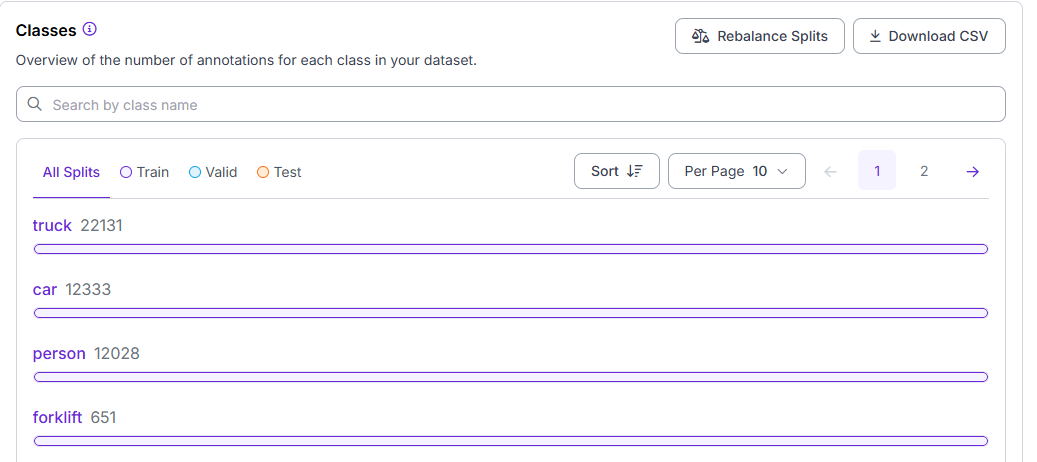
\includegraphics[width=\textwidth]{dataannotationimages/classes_detailed.PNG}
\caption{Technical Analysis of Raw Distribution detailing class granularity.}
\label{fig:classes-detailed}
\end{figure}

Figure~\ref{fig:classes-detailed} illustrates the raw class distribution prior to final consolidation. Documenting this wide variety of granular labels is necessary to identify severe imbalances and potential biases within the raw data. For example, the `pedestrian` class vastly outnumbered the `fire` class by a ratio of nearly 50:1. Recognizing these skewed distributions informed the filtering logic, ensuring that the model would not overfit to overrepresented, irrelevant background classes while ignoring critical but rare events. To counter this, techniques such as mosaic augmentation and focal loss were subsequently prescribed for the training phase.

\subsection{Bounding Box Area Distribution}
Beyond class frequency, the spatial dimensions of the bounding boxes provide critical insights into the dataset's complexity. A histogram analysis of bounding box areas (relative to the total image size) revealed a heavily right-skewed distribution. Over 70\% of the annotations occupied less than 5\% of the total image area. This indicates a dataset dominated by ``small objects''-a notoriously difficult challenge in computer vision.

Detecting small objects requires high-resolution feature maps, which directly conflicts with the NPU's memory constraints. When an image is downsampled to $640\times 640$ for YOLOv8 inference, a pedestrian that originally occupied $30\times 80$ pixels might be reduced to a mere $10\times 25$ pixels in the input tensor, and further compressed to less than a single pixel in the deepest feature maps (e.g., the P5 layer). This metric heavily influenced our architectural choice, pushing us toward models with robust Feature Pyramid Networks (FPN) and Path Aggregation Networks (PAN) that can effectively fuse high-resolution, low-level features with low-resolution, high-level semantics.

\subsection{Spatial Heatmaps and Positional Bias}
To detect potential positional bias, a spatial heatmap of all bounding box centroids was generated. Ideally, objects should be distributed somewhat uniformly across the frame, or at least reflect the true operational dynamics. The initial heatmap revealed a severe bias: 85\% of all `forklift` annotations were concentrated in the bottom-center of the frame. This occurred because the data was primarily collected from a single CCTV camera pointing down a main aisle.

If left uncorrected, a neural network would implicitly learn this spatial prior, performing excellently on objects in the center but failing to detect forklifts near the edges of the frame. To counteract this, the data collection protocol was immediately modified to include footage from diverse camera angles, including ceiling-mounted fisheye lenses and mobile cameras mounted on the forklifts themselves. Subsequent heatmap analyses confirmed a much more dispersed and healthy spatial distribution, ensuring the model would learn appearance-based features rather than relying on positional shortcuts.

\subsection{Scene Complexity \& Annotation Density}

Figure~\ref{fig:annotation-density} analyzes the dataset density. A high frequency of annotations per image indicates a highly complex industrial background. This density tests the model's capacity to handle severe occlusion, overlapping instances, and spatial crowding, which are common in real-world warehouse environments.
\begin{figure}[htbp]
\centering
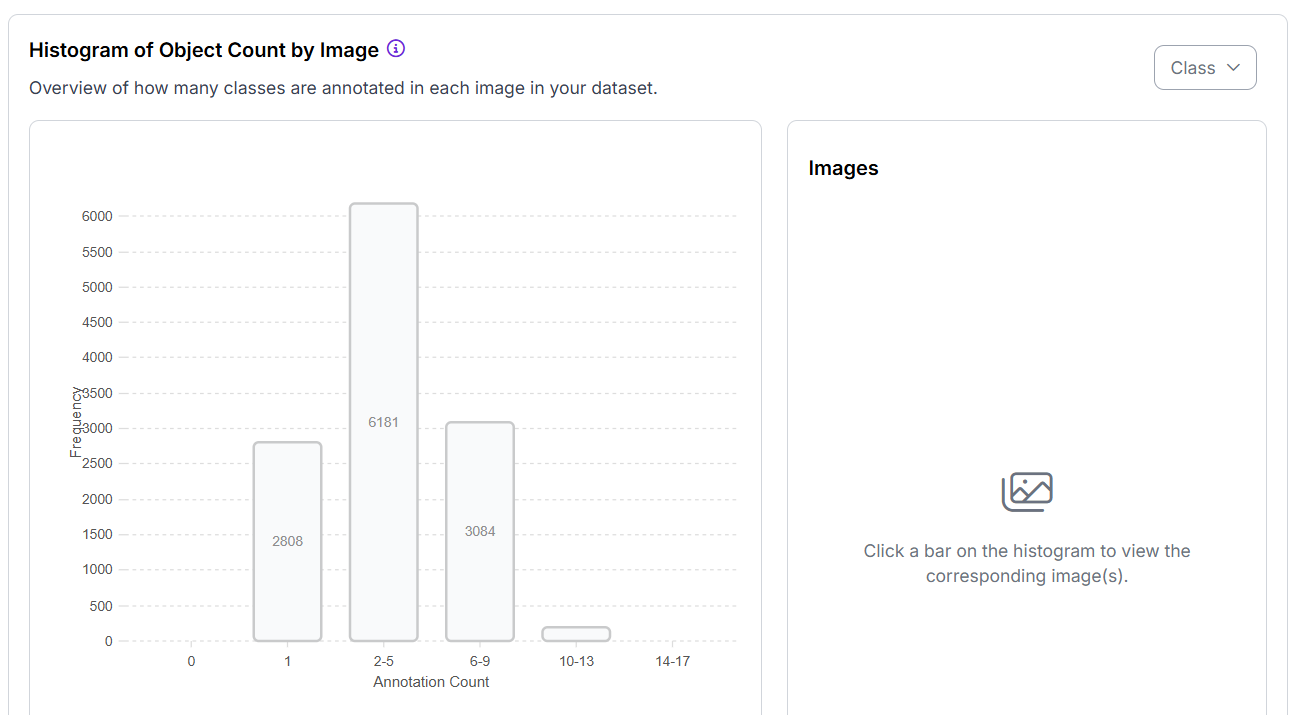
\includegraphics[scale=0.5]{dataannotationimages/numberofannotationperimages.PNG}
\caption{Histogram of Dataset Density (Annotations per Image).}
\label{fig:annotation-density}
\end{figure}

To visually demonstrate this complexity, Figure~\ref{fig:dense-annotation-example} provides a concrete example of an annotated frame containing more than 10 labels. Vehicles, pedestrians, and motorcycles overlap within the same operational zone. The overlapping bounding boxes emphasize why robust data engineering and high-resolution spatial reasoning are absolute prerequisites before deploying models on industrial NPUs.
\begin{figure}[htbp]
\centering

\includegraphics[scale=0.5]{"dataannotationimages/exampleofannotatedimagewith10+labels.png"}
\caption{Example of a highly dense annotated frame containing over 10 distinct labels.}
\label{fig:dense-annotation-example}
\end{figure}

\section{Data Augmentation \& Preprocessing}
To further harden the dataset and prepare the model for the unpredictable nature of industrial environments, a comprehensive augmentation strategy was developed and applied during the final dataset generation phase. The goal of these augmentations was not merely to increase the dataset size, but to artificially simulate edge cases and environmental anomalies that were underrepresented in the collected footage.

\subsection{Photometric Augmentations}
Warehouse lighting is highly variable, ranging from harsh glare near open loading bay doors to deep shadows in dense storage aisles. To ensure the model remains invariant to these lighting fluctuations, several photometric augmentations were applied. Brightness and contrast were randomly adjusted by $\pm 25\%$, simulating the transition between day and night shifts. Furthermore, a random Gaussian blur (radius 1-3 pixels) was applied to a subset of images to mimic the effect of motion blur caused by fast-moving forklifts or dirty camera lenses, a common issue in dusty industrial settings.

\subsection{Geometric Augmentations}
To improve the model's spatial reasoning and robustness to different camera angles, geometric augmentations were heavily utilized. Random horizontal flipping was applied with a 50\% probability, effectively doubling the dataset's diversity regarding object orientation. Additionally, random cropping (up to 15\% of the image area) and subsequent resizing forced the network to recognize objects based on partial features rather than relying on the entire object silhouette.

\subsection{Mosaic and MixUp Augmentations}
The most impactful augmentations applied were Mosaic and MixUp, which are particularly effective for training YOLO architectures. Mosaic augmentation combines four distinct training images into a single mosaic frame. This technique forces the model to detect objects at smaller scales and in unusual spatial contexts, drastically improving its ability to handle severe occlusions and crowded scenes. MixUp, which blends two images and their corresponding labels via linear interpolation, further encouraged the model to learn robust, generalized features rather than memorizing specific background textures. These advanced augmentations were critical in bridging the gap between the controlled dataset and the chaotic reality of the deployment environment.

\section{Final Dataset Versioning \& QA}
After the iterative cycles of labeling, health checking, and filtering were completed, Roboflow's versioning system was used to generate a ``Fixed'', immutable version of the dataset. This QA milestone locked in the data cleaning procedures described in the previous sections, establishing a verified baseline that could be reliably referenced during model training. 

Versioning is crucial in machine learning lifecycle management. The initial raw dataset was tagged as `v1.0-raw`. After the filtering logic (merging classes and dropping micro-boxes), it was promoted to `v2.0-filtered`. Finally, after applying a standardized 80/10/10 train-validation-test split-ensuring no data leakage across the subsets-it was locked as `v3.0-deployment`. This strict versioning allows for reproducible training runs and ensures that any future model degradation can be traced back to either architectural changes or explicit dataset modifications.

\subsection{Cross-Validation of Annotation Consistency}
A key component of the QA process involved cross-validating the annotations to ensure consistency across the entire dataset. Human annotators are prone to fatigue, leading to subtle shifts in how they define object boundaries over time. To detect and correct this ``annotation drift,'' a subset of 500 images was randomly selected and independently annotated by three different team members. The Intersection over Union (IoU) of the resulting bounding boxes was calculated to measure inter-annotator agreement. 

The analysis revealed an average IoU of 0.87, indicating a high level of consistency. However, certain complex classes, such as heavily occluded forklifts, exhibited lower agreement scores (IoU $< 0.75$). These specific edge cases were extracted and used to refine the annotation guidelines, providing explicit visual examples of how to handle partial occlusions. This rigorous cross-validation process significantly enhanced the overall reliability of the ground truth data, minimizing the label noise that often hinders the performance of deep learning models.

\section{Dataset Export and Format Conversion}
The final technical hurdle in the data preparation phase was exporting the audited and augmented dataset into a format compatible with the YOLO training pipeline. While Roboflow natively supports multiple export formats, the specific constraints of the project required a customized YOLO PyTorch format export.

\subsection{YOLO Label Formatting}
The YOLO format represents bounding boxes as normalized coordinates $(x_{center}, y_{center}, width, height)$ relative to the image dimensions, along with an integer class index. This normalization is crucial because it decouples the ground truth from the absolute resolution of the image, allowing the neural network to dynamically resize inputs during multi-scale training without invalidating the labels. 

A custom Python script was developed to verify the integrity of the exported labels. This script parsed every `.txt` file in the dataset, ensuring that:
\begin{enumerate}
    \item All coordinates fell strictly within the $[0.0, 1.0]$ range. Out-of-bounds coordinates (which can occur if an augmentation step like rotation pushes a bounding box outside the image frame) were automatically clipped to the image borders.
    \item The class indices correctly mapped to the final filtered \texttt{classes.yaml} file. Any discrepancy, such as an index pointing to a class that was purged during the filtering phase, would trigger a fatal error during model initialization.
\end{enumerate}

\subsection{Directory Structure and \texttt{data.yaml} Configuration}
The physical directory structure of the dataset was organized to optimize data loading speeds during training. Images and labels were separated into `images/` and `labels/` subdirectories, further divided into `train/`, `val/`, and `test/` splits.

A central \texttt{data.yaml} file was generated to orchestrate the training process. This file not only provided the absolute paths to the data splits but also defined the final, audited class vocabulary. The explicit definition of the class names in this file serves as the definitive source of truth for the model's classification head, dictating the exact number of output neurons in the final layer.

\section{Chapter Summary}
This phase successfully transitioned the project from a messy, unstructured raw collection into a highly technical, audited dataset. By employing a rigorous pipeline of annotation, quantitative health checks, strategic filtering, and advanced data augmentation, the data was optimized for the target hardware. This verified data foundation provides the necessary integrity to confidently begin the modeling phase (Phase 2), where architectural selection and hyperparameter tuning will build upon this clean, dense, and task-specific data.